\documentclass{beamer}

\usepackage[english,UKenglish]{babel}
\usepackage{tikz}
\usepackage{datetime}

\newcommand{\image}[2][]{%
  \IfFileExists{#2}%
    {\includegraphics[#1]{#2}}%
    {%
      \begingroup\fboxsep=-\fboxrule
      \fbox{%
        \rule{150pt}{0pt}%
        \rule{0pt}{100pt}%
      }%
      \endgroup%
    }%
}

\newdate{swat_pres_date}{16}{05}{2014}

\definecolor{cwi-red}{cmyk}{0,.9058,.7068,.251}
\definecolor{cwi-blue}{cmyk}{.7,.4,.4,0}
\definecolor{cwi-green}{cmyk}{.41,.18,.43,.1}
\definecolor{cwi-orange}{cmyk}{.14,.35,.65,.15}
\definecolor{cwi-yellow}{cmyk}{.14,.20,.65,.16}

\usetheme{Madrid}
\useinnertheme{rectangles}
\usecolortheme[named=cwi-blue]{structure}
\setbeamertemplate{blocks}[default]
\beamertemplatenavigationsymbolsempty

\setbeamertemplate{caption}{%
  \scriptsize%
    {\usebeamercolor[fg]{section in toc}\insertcaptionname\ \insertcaptionnumber:}%
    \ \insertcaption%
}

\newlength{\wideitemsep}
\setlength{\wideitemsep}{\itemsep}
\addtolength{\wideitemsep}{.6em}
\let\olditem\item
\renewcommand{\item}[1][\wideitemsep]{\setlength{\itemsep}{#1}\olditem}
\def\sitem{\item[.2em]}

\title[Interaction Design for Molecule Param.]{Interaction Design for Fragment-Based Molecule Parameterisation}
\author[Jimi van der Woning]{Jimi M. van der Woning\\\url{Jimi.vanderWoning@student.uva.nl}}
\institute[UvA, CWI]{\parbox{4.1cm}{\center\scshape\includegraphics[height=1.5cm]{uva_logo}\\[.1cm]University of Amsterdam} \parbox{.5cm}{\center\vspace{1.5cm}\ \\[.1cm]and} \parbox{5.2cm}{\center\scshape\includegraphics[height=1.5cm]{cwi_logo}\\[.1cm]Centrum Wiskunde \& Informatica}\\[1cm]{\bf Supervisors:} Mohammed El-Kebir, Gunnar W. Klau, and Tijs van der Storm}
\date{\displaydate{swat_pres_date}}




\begin{document}

\setlength{\itemsep}{20pt}



\begin{frame}
\titlepage
\end{frame}



\addtobeamertemplate{frametitle}{\let\insertframetitle\insertsectionhead\let\insertframesubtitle\insertsubsectionhead}{%
\begin{tikzpicture}[remember picture,overlay]
\node[anchor=north east,yshift=2pt] at (current page.north east) {\includegraphics[height=0.8cm]{cwi_logo}};
\node[anchor=north east,yshift=2pt,xshift=-2cm] at (current page.north east) {\includegraphics[height=0.8cm]{uva_logo}};
\end{tikzpicture}}



\section*{Contents}
\begin{frame}{x}{}
\setcounter{tocdepth}{1}
\tableofcontents
\end{frame}



\section{Introduction}
\subsection{Chemical concepts}
\begin{frame}{x}{}
  \begin{columns}
   \column{0.4\textwidth}
     \begin{figure}
      \centering
      \image[width=\textwidth]{img/molecule.pdf}
      \caption{Ethanamine molecule~\cite{atb2014ethanamine}.}
     \end{figure}
  
   \column{0.5\textwidth}
    \begin{itemize}
      \item Everything consists of molecules;
      \item Molecules consist of atoms and bonds;
      \item Atoms have a charge;
      \item Atoms can be grouped in charge groups.
    \end{itemize}
  \end{columns}
\end{frame}


\subsection{Problem analysis}
\begin{frame}{x}{}
  \begin{columns}
   \column{0.3\textwidth}
    \begin{itemize}
     \item<1-> Current methods are too slow;
     \item<2-> Possible to parameterise a molecule based on fragments of other molecules;
     \item<3-> No existing software for this.
    \end{itemize}

   \column{0.6\textwidth}<2->
    \begin{figure}
     \vspace{-1em}
     \frame{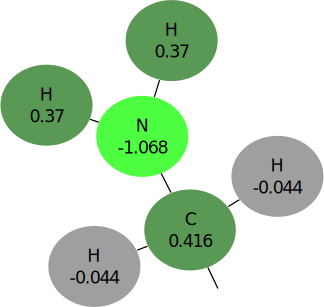
\includegraphics[width=.42\textwidth]{img/match_target.pdf}}%
     \\[.3cm]
     \frame{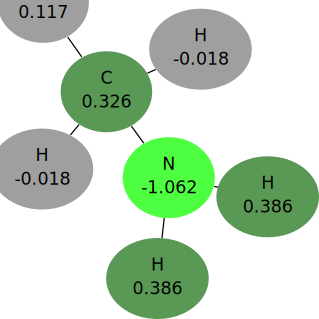
\includegraphics[width=.42\textwidth]{img/match_good.pdf}}%
     \qquad
     \frame{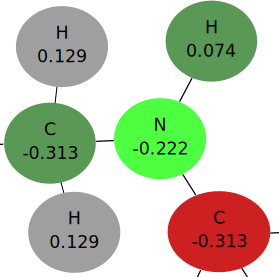
\includegraphics[width=.42\textwidth]{img/match_none.pdf}}
     \vspace{-.2cm}
     \caption{Fragment matching.}
    \end{figure}
  \end{columns}
\end{frame}



\section{Approach}
\begin{frame}{x}{}
\begin{itemize}
\item<1-> Design and implement two versions:
      \begin{itemize}
      \sitem Consuming: non-automated;
      \sitem Producing: semi-automatic.
      \end{itemize}
\item<2-> Compare in a user study:
      \begin{itemize}
      \sitem Parameterise molecules in both versions;
      \sitem Positive SUS / UMUX questionnaire;
      \sitem General questionnaire.
      \end{itemize}
\end{itemize}
\end{frame}



\section{Hypotheses}
\begin{frame}{x}{}
\begin{itemize}
\item<1-> It is possible to parameterise a molecule based on fragments of other molecules; both correctly and in a reasonable amount of time.
\item<2-> The producing version will take the least time to use.
\item<3-> The consuming version will yield more accurate results.
\item<4-> For a tool for fragment-based molecule parameterisation, it is better for users to have full, manual control, than to automate certain parts.
\end{itemize}
\end{frame}



\section{Interaction Design}
\begin{frame}{x}{}
 \begin{columns}
  \column{.45\textwidth}
   \begin{block}{Consuming version}
    \begin{enumerate}
     \item<2-> Insert a molecule;
     \item<3-> Select atom(s);
     \item<4-> Compare fragments;
     \item<5-> Pick a fragment;
     \item<9-> Fine-tune charges;
     \item<10-> Download result.
    \end{enumerate}
   \end{block}

  \column{.45\textwidth}
   \begin{block}{Producing version}
    \begin{enumerate}
     \item<2-> Insert a molecule;
     \item<6-> Click ``Start'' button;
     \item<7-> Inspect suggested fragment;
     \item<8-> Accept/Reject fragment;
     \item<9-> Fine-tune charges;
     \item<10-> Download result.
    \end{enumerate}
   \end{block}

 \end{columns}
\end{frame}



\section{Implementation}
\begin{frame}{x}{}
TODO:
\begin{itemize}
\item Create this slide\ldots
\end{itemize}
\end{frame}



\section{Results}
\subsection{Time consumption}
\begin{frame}{x}{}
TODO:
\begin{itemize}
\item Create this slide\ldots
\end{itemize}
\end{frame}


\subsection{Result accuracy}
\begin{frame}{x}{}
TODO:
\begin{itemize}
\item Create this slide\ldots
\end{itemize}
\end{frame}


\subsection{Usability rating}
\begin{frame}{x}{}
TODO:
\begin{itemize}
\item Create this slide\ldots
\end{itemize}
\end{frame}


\subsection{Comments}
\begin{frame}{x}{}
TODO:
\begin{itemize}
\item Create this slide\ldots
\end{itemize}
\end{frame}


\subsection{Future work}
\begin{frame}{x}{}
TODO:
\begin{itemize}
\item Create this slide\ldots
\end{itemize}
\end{frame}



\section{Conclusion}
\begin{frame}{x}{}
TODO:
\begin{itemize}
\item Create this slide\ldots
\end{itemize}
\end{frame}



\section*{Bibliography}
\begin{frame}[allowframebreaks]{x}{}
\nocite{all, the, things}
\bibliographystyle{abbrv}
\tiny{\bibliography{../thesis/references}}
\end{frame}



\end{document}
